\chapter{Theoretical Analysis} \label{chap:theoretical-analysis}
\section{Constant Velocity}
\subsection{Dirichlet Boundary}
If we set the velocity profile of the equilibrium flow to constant $v_0=\text{const}$, then Eq.(\ref{eq:polynomial-eigenvalue-problem}) becomes a simple boundary value problem with second order constant coefficients differential equation.

\begin{equation} \label{eq:constant-v-problem-dirichlet}
    \omega^2\tilde{v} + 2i\omega v_0\pdv{\tilde{v}}{z} + (1-v_0^2)\pdv[2]{\tilde{v}}{z} = 0
    \quad
    \tilde{v}(-1) = \tilde{v}(1) = 0
\end{equation}

The solution to this problem is
\begin{equation} \label{eq:constant-v-solution-dirichlet}
    \tilde{v} = \exp\left(-\frac{i\omega}{v_0+1}\right)
\left[ \exp\left(i\omega\frac{z+1}{v_0+1}\right) - \exp\left(i\omega\frac{z+1}{v_0-1}\right) \right], \quad \omega=n\pi(1-v_0^2)/2 \in \mathbb{R}.
\end{equation}

This result tells us for constant velocity case, the flow in magnetic nozzle is stable regardless the velocity $v_0$. It is worth to mention $v_0=1$ is a singular point of this problem.

We will use this to benchmark the experimental results. 

\begin{figure}[H]
	\centering
	\begin{subfigure}{0.5\textwidth}
		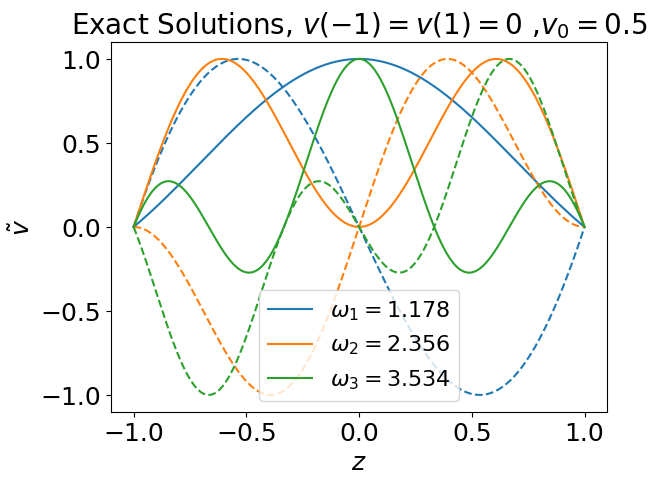
\includegraphics[width=\linewidth]{img/theoretical-analysis/exact-fixed-fixed-v0=0.5}
		\caption{Subsonic}
	\end{subfigure}%
	\begin{subfigure}{0.5\textwidth}
		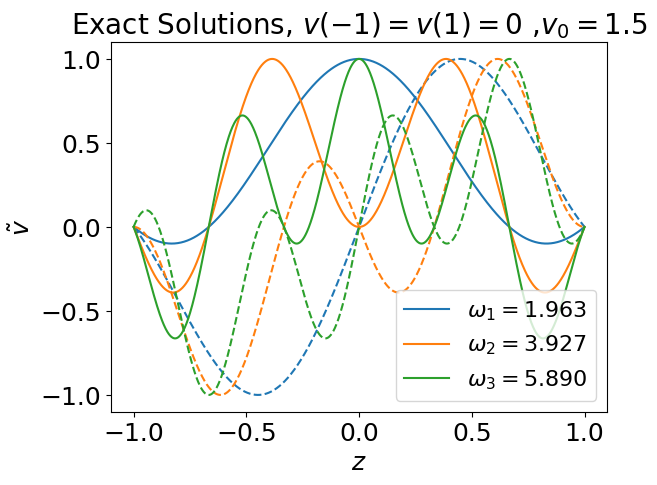
\includegraphics[width=\linewidth]{img/theoretical-analysis/exact-fixed-fixed-v0=1.5}
		\caption{Supersonic}
	\end{subfigure}
	\caption{The plots show the first three non-zero exact solutions to Eq.(\ref{eq:constant-v-problem-dirichlet}) for both subsonic and supersonic case. These solutions are stable.}
	\label{fig:exact-v-dirichlet}
\end{figure}

\subsection{Fixed-Open Boundary}

\begin{equation} \label{eq:constant-v-problem-fixed-open}
	\omega^2\tilde{v} + 2i\omega v_0\pdv{\tilde{v}}{z} + (1-v_0^2)\pdv[2]{\tilde{v}}{z} = 0
	\quad
	\tilde{v}(-1) = \pdv{\tilde{v}}{z}\,(1) = 0
\end{equation}

The solution to this problem is
\begin{equation} \label{eq:constant-v-solution-fixed-open}
	\begin{aligned}
		\tilde{v} &= \exp\left(-\frac{i\omega}{v_0+1}\right)
		\left[ \exp\left(i\omega\frac{z+1}{v_0+1}\right) - \exp\left(i\omega\frac{z+1}{v_0-1}\right) \right], \\
		\omega &= (v_0^2 - 1) \left[\frac{n\pi}{2} - \frac{1}{4}i\ln(\frac{v_0-1}{v_0+1})\right]
	\end{aligned}
\end{equation}
For any $v_0\neq 1$, the term $i\ln((v_0-1)/(v_0+1))\in\mathbb{C}$ and its imaginary part is positive. Therefore,
\begin{itemize}
	\item If $v_0<1$, then $\Im(\omega)<0$, it's damped oscillation.
	\item If $v_0>1$, then $\Im(\omega)>0$, it's unstable.
\end{itemize}

Worth to mention, this is a very interesting solution with the following properties,
\begin{enumerate}
	\item The growth rate is independent the mode number $n$.
	\item The ground mode $n=0$ for subsonic case has non-zero real part and imaginary part.
\end{enumerate}

\begin{figure}[H]
	\centering
	\begin{subfigure}{0.5\textwidth}
		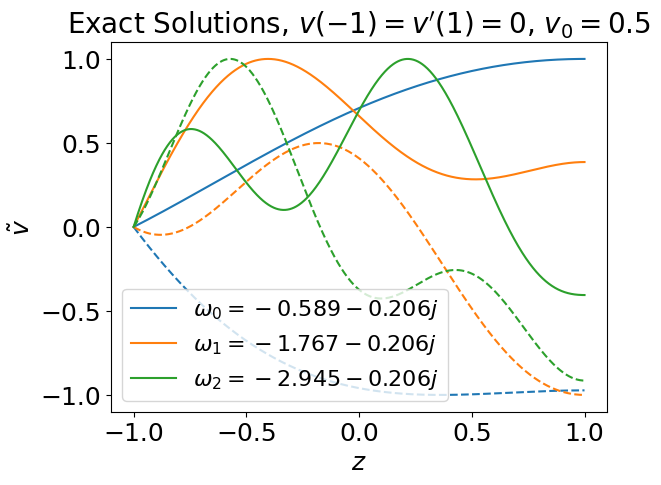
\includegraphics[width=\linewidth]{img/theoretical-analysis/exact-fixed-open-v0=0.5}
		\caption{Subsonic, stable flow.}
	\end{subfigure}%
	\begin{subfigure}{0.5\textwidth}
		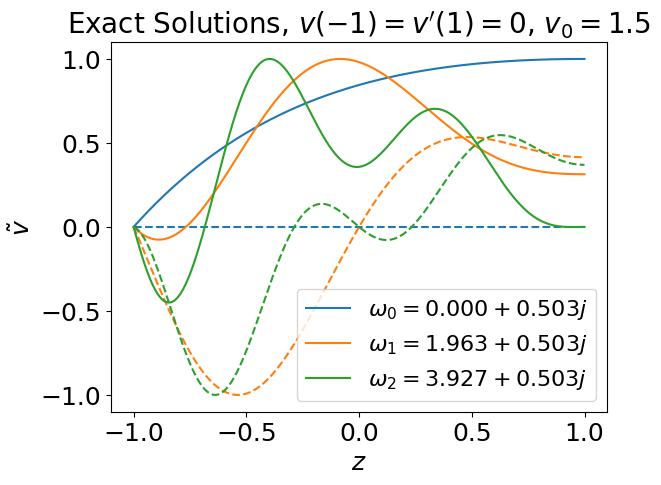
\includegraphics[width=\linewidth]{img/theoretical-analysis/exact-fixed-open-v0=1.5}
		\caption{Supersonic, unstable flow.}
	\end{subfigure}
	\caption{The plots show the first three exact solutions to Eq.(\ref{eq:constant-v-problem-fixed-open}) for both subsonic and supersonic case. The flow is stable for subsonic case and unstable for supersonic case.}
	\label{fig:exact-v-fixed-open}
\end{figure}


\section{Spectral Pollution and Spurious Modes}
In this section, we will discuss an important phenomenon we will observe throughout the numerical experiments. It is the phenomenon of spectral pollution.

Spectral pollution refers to the phenomenon which some eigenvalues are not converging to the correct value when the mesh density is increased. When solving eigenvalue problems using spectral methods with finite difference or finite element approximations, spectral pollution might occur. \cite{llobet_spectral_1990}

\subsection{Finite Difference Discretization of Operators}
In this section, we are going to investigate the spectral pollution phenomenon when solving Eq.(\ref{eq:constant-v-problem-dirichlet}) using spectral method.

The dispersion relation can be obtained by substituting $\tilde{v} = \exp(-i\omega t + kx)$ into Eq.(\ref{eq:constant-v-problem-dirichlet}),
\begin{equation} \label{dispersion-relation}
	\omega = k(v_0 \pm 1) 
\end{equation}

If we assume $v\sim \exp(ikx)$, and let $\beta\equiv kh/2$. Then in finite difference discretization scheme, the differential operators $\dv*[n]{z}$ are equivalent to the following factors \cite{llobet_spectral_1990},
\begin{align}
	&G_0 = 1 \nonumber \\
	&G_1 = [\exp(2i\beta)-\exp(-2i\beta)]/2h = (i/h)\sin(2\beta) 
	\label{G-operator}\\
	&G_2 = [\exp(2i\beta)-2-\exp(-2i\beta)]/h^2 = (2/h^2)(\cos(2\beta)-1) \nonumber 
\end{align}


\subsection{Analysis of Numerical Spectrum}
\subsubsection{Discretize on the Same Grid}
Using the G-operator, Eq.(\ref{G-operator}), the discretized equation of Eq.(\ref{eq:constant-v-problem-dirichlet}) is 
\begin{equation} \label{eq:discretized-eq-G}
    (\omega^2G_0 + \omega G_1 + G_2)\mathbf{\tilde{v}} = 0
\end{equation}
where $\mathbf{\tilde{v}}$ is the discretized vector of $\tilde{v}$.

Solving Eq.(\ref{eq:discretized-eq-G}), we obtain the numerical dispersion relation,
\begin{equation} \label{dispersion-relation-G}
	\omega = \frac{2\sin(\beta)}{h}\left(v_0 \pm \sqrt{1 - v_0^2\sin[2](\beta)}\right)
\end{equation}

Given $h$ (fixed the mesh resolution), we see that
\begin{itemize}
	\item $\omega$ is real for all $k$ if $v_0 < 1$.
	\item $\omega$ is complex for large $k$, more specifically $k>h/2\arcsin(1/v_0)$, if $v_0 > 1$.
	\item For small $k$, meaning $k\to 0$, Eq.(\ref{dispersion-relation-G}) is a good representation for the analytical dispersion relation, Eq.(\ref{dispersion-relation}). 
\end{itemize}
This explains why the spurious unstable modes occur when $v_0>1$.

\begin{figure}[H]
	\centering
	\begin{subfigure}[b]{0.5\linewidth}
		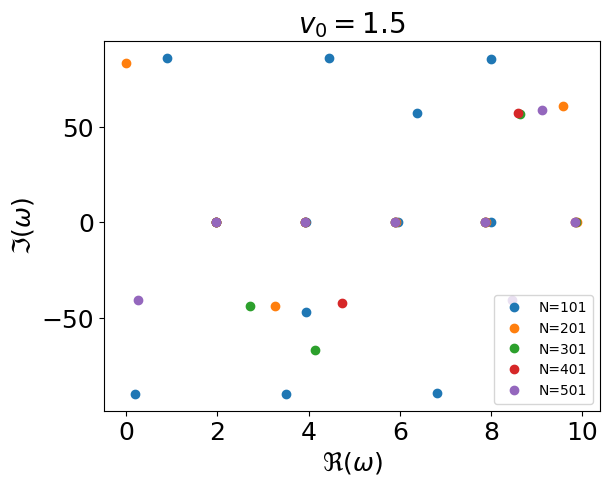
\includegraphics[width=\linewidth]{img/theoretical-analysis/eigvals-bad} 
		\caption{Bad eigenvalues}
	\end{subfigure}%
	\begin{subfigure}[b]{0.5\linewidth}
		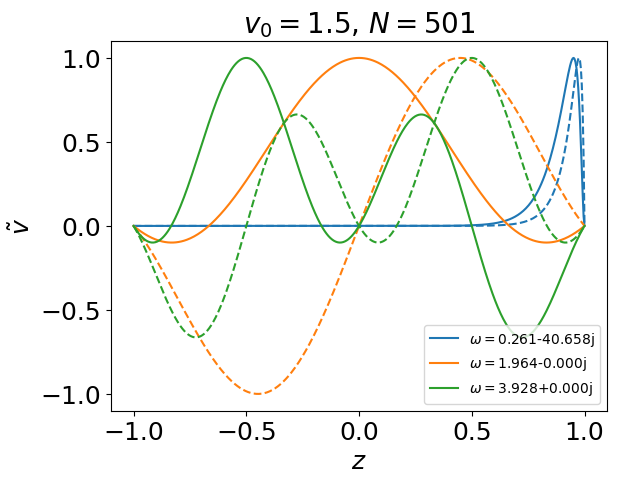
\includegraphics[width=\linewidth]{img/theoretical-analysis/eigvecs-bad} 
		\caption{Bad eigenfunctions}
	\end{subfigure}
	\caption{Spurious modes.}
	\label{fig:results-bad}
\end{figure}

One way to filter the spurious modes is to remove all modes with $k>h/2 \arcsin(1/v_0)$, see Fig.\ref{fig:results_filter_k}. However, this is not a good way to deal with general cases because it requires the solution to the discretized problem Eq.(\ref{eq:discretized-eq-G}). For general problem with non-constant velocity profile, it is hard to solve the discretized problem directly.

\begin{figure}[H]
	\centering
	\begin{subfigure}[b]{0.5\linewidth}
		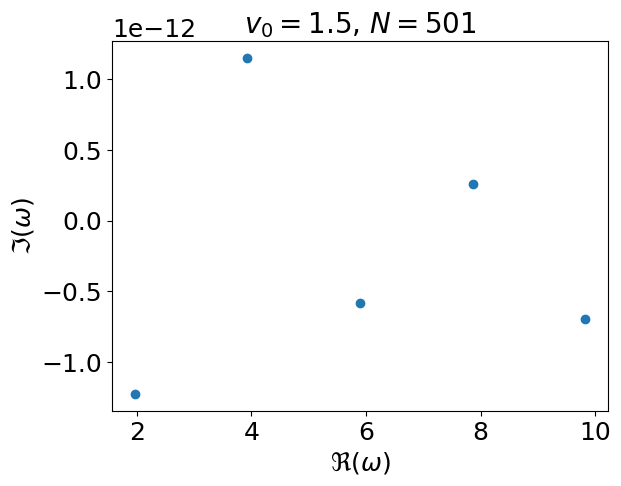
\includegraphics[width=\linewidth]{img/theoretical-analysis/eigvals-good} 
		\caption{Good eigenvalues}
	\end{subfigure}%
	\begin{subfigure}[b]{0.5\linewidth}
		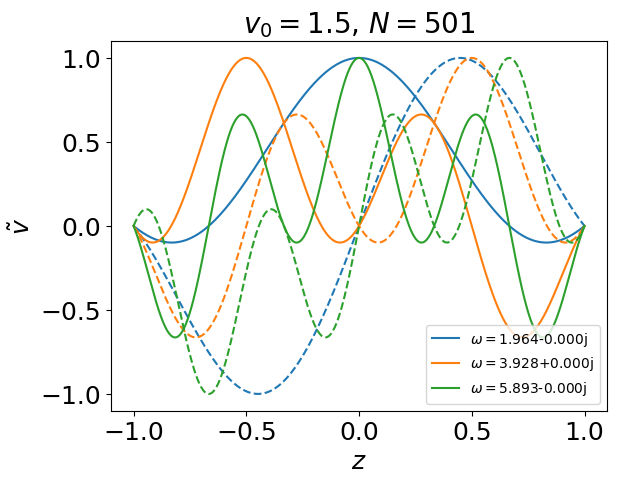
\includegraphics[width=\linewidth]{img/theoretical-analysis/eigvecs-good} 
		\caption{Good eigenfunctions}
	\end{subfigure}
	\caption{Filter out the spurious modes with $k>h/2\arcsin(1/v_0)$.}
	\label{fig:results-filter-k}
\end{figure}

A better way to filter the spurious modes is by doing a "convergence test". Since the frequency Eq.(\ref{dispersion-relation-G}) is changing with mesh resolution $h$. We can simply solve the discretized problem using spectral method under different mesh resolution. Then filter out the eigenmodes that are changing dramatically.

\section{Symmetry of Growth Rates in Accelerating and Decelerating Cases}
Notice that there exists a symmetry between the accelerating and decelerating velocity profiles. To be specific, these two profiles are symmetric about the axis $z=0$.
\[ v_a(-z) = v_d(z) \]
where the subscript $a$ stands for accelerating and $d$ stands for decelerating.

The symmetry between the two velocity profiles will lead us to the symmetry of growth rates between the accelerating case and decelerating case. 

\begin{proposition} \label{prop:symmetry-of-eigenvalue}
	If $\omega$ is an eigenvalue to the polynomial eigenvalue problem, Eq.\ref{eq:polynomial-eigenvalue-problem} width accelerating velocity profile $v_a(z)$, then its complex conjugate, $\overline{\omega}$, is an eigenvalue to the same equation with decelerating velocity profile, $v_d(z)$.
\end{proposition}
\begin{proof}
	Suppose $\omega=\omega_r + i\omega_i$ is an eigenvalue to Eq.\ref{eq:polynomial-eigenvalue-problem}. Substitute $\tilde{v}(z)$ by $\exp(ikz)$ and split the equation to real and imaginary part, we see that $\omega$ and $\omega_i$ must satisfy
	\begin{equation} \label{eq:eigenvalue-problem-real-part}
		\omega_r^2 - \omega_i^2 
		- 2\omega_r kv_0 - 2\omega_i\pdv{v_0}{z}
		+ \left[
		-k^2(1-v_0^2) 
		-\left(1-\frac{1}{v_0^2}\right)\left(\pdv{v_0}{z}\right)^2
		-\left(v_0+\frac{1}{v_0}\right)\pdv[2]{v_0}{z}
		\right]
		= 0
	\end{equation}
	\begin{equation} \label{eq:eigenvalue-problem-imag-part}
		2\omega_r\omega_i 
		- 2\omega_i kv_0 + 2\omega_r\pdv{v_0}{z} 
		- k\left(3v_0+\frac{1}{v_0}\right)\pdv{v_0}{z} 
		= 0
	\end{equation}
	Here the velocity profile $v_0$ can be accelerating, $v_a$, or decelerating, $v_d$.
	
	Since $v_d(z)=v_a(-z)$, so $\partial_zv_d=-\partial_zv_a$ and $\partial_z^2v_d=\partial_z^2v_a$. If the transformation $z\to -z$ is made, then Eq.\ref{eq:eigenvalue-problem-real-part} and Eq.\ref{eq:eigenvalue-problem-imag-part} become
	
	\[
		\omega_r^2 - \omega_i^2 
		- 2\omega_r kv_0' + 2\omega_i\pdv{v_0'}{z}
		+ \left[
		-k^2(1-v_0'^2) 
		-\left(1-\frac{1}{v_0'^2}\right)\left(\pdv{v_0'}{z}\right)^2
		-\left(v_0'+\frac{1}{v_0'}\right)\pdv[2]{v_0'}{z}
		\right]
		= 0
	\]
	\[
		2\omega_r\omega_i 
		- 2\omega_i kv_0' - 2\omega_r\pdv{v_0'}{z} 
		- k\left(3v_0'+\frac{1}{v_0'}\right)\pdv{v_0'}{z} 
		= 0
	\]
	where $v_0'(z) \equiv v_0(-z)$. We see that the imaginary part of the eigenvalue changes from $\omega_i$ to $-\omega_i$.
\end{proof}

\begin{remark}
	This proposition tells us that if the flow in magnetic nozzle is unstable in one case, then the flow will stable in the opposite case. More specifically, the perturbation is damped oscillation.
\end{remark}

